\section{Challenge 4: Ακολούθηση διαδρομής και αποφυγή εμποδίων με τη χρήση αισθητήρων laser}\label{section:ex4}
Σε αυτό το ερώτημα καλούμαστε να συνδυάσουμε τον κώδικα από τα \ref{section:ex1} και \ref{section:ex3} έτσι ώστε το όχημά μας να μπορεί να ακολουθεί ένα δοσμένο target και συγχρόνως να αποφεύγει τα εμπόδια του χάρτη.
Όπως και στο ερώτημα~\ref{section:ex1} χρησιμοποιείται η motor schema στρατηγική από την \cite{etsardou-phd} με τις σχέσεις \ref{eq:u} και \ref{eq:omega}.
Το αρχείο στο οποίο πρέπει να συμπληρωθεί ο κώδικας είναι το
\url{art_autonomous_exploration/src/speeds_assignment.py}.

Ο κώδικας του project τροποποιήθηκε έτσι ώστε αν αποφευχθεί η ύπαρξη των ίδιων υπολογισμών σε δύο σημεία.
Έτσι, η διαφορά  είναι ότι οι συντελεστές \mintinline{python}!linear! και \mintinline{python}!angular! υπολογίζονται με την κλίση της \mintinline{python}!velocitiesToNextSubtarget()!
ενώ στην ενότητα~\ref{section:ex1} ήταν \mintinline{python}!1! και \mintinline{python}!0! αντίστοιχα.

Εδώ, οι συντελεστές $c_u = 0.0001$ και $c_w = 0.0005$ παίρνουν μικρότερη τιμή καθώς θέλουμε να επηρεάζουν λιγότερο τη κίνηση του ρομπότ.
Επίσης, σημειώνεται ότι $c_u < c_w$ καθώς προτιμάμε να έχουμε στροφή του ρομπότ παρά σημαντική μείωση της ταχύτητας του κοντά στα εμπόδια.

Ένα πρόβλημα που συναντήθηκε με αυτό το μοντέλο είναι η πιθανότητα μηδενισμού της ταχύτητας του ρομπότ όταν η ταχύτητες αποφυγής έχουν αντίθετο πρόσημο με τις ταχύτητες από το target.
Όταν οι ταχύτητες παίρνουν πολύ χαμηλές τελικές τιμές το όχημα ακινητοποιείται και δεν υπάρχει τρόπος να αναπτύξει ταχύτητα μέχρι να περάσει το χρονικό όριο και να ανατεθεί νέα διαδρομή.
Μια ευριστική προσέγγιση σε αυτό το πρόβλημα είναι να θέτουμε ταχύτητες στο ρομπότ με τα πρόσημα των ταχυτήτων αποφυγής, έτσι ώστε το ρομπότ να μη ``πέσει'' πάνω σε εμπόδιο και να κουνηθεί από τη θέση του.
Εφόσον ικανοποιηθεί η αρχική συνθήκη (μικρές τελικές ταχύτητες του ρομπότ) εφαρμόζουμε αυτή τη στρατηγική για έναν συνεχόμενο αριθμό επαναλήψεων.
Ο σχετικός κώδικας:
\begin{code}
\caption{Σε περίπτωση μηδενισμού της ταχύτητας θέτουμε νέες ταχύτητες σύμφωνα με τα πρόσημα των ταχυτήτων αποφυγής}
\begin{pythoncode}
if self.stuck_count or (abs(linear) + abs(angular) < (self.MAX_LINEAR_VELOCITY + self.MAX_ANGULAR_VELOCITY) / 2 / 6):
    linear = self.MAX_LINEAR_VELOCITY * np.sign(l_laser) / 2
    angular = self.MAX_ANGULAR_VELOCITY * np.sign(a_laser)
    self.stuck_count = 0 if self.stuck_count >= self.STUCK_LIMIT else self.stuck_count + 1
\end{pythoncode}
\end{code}
Η στρατηγική αυτή παράγει μικτά αποτελέσματα και επιδέχεται βελτίωση.
Θα μπορούσαν για παράδειγμα να συμπεριληφθούν τα δεδομένα από το sonar ώστε να καλύπτονται και τα εμπόδια πίσω από το ρομπότ.

\begin{figure}
    \centering
    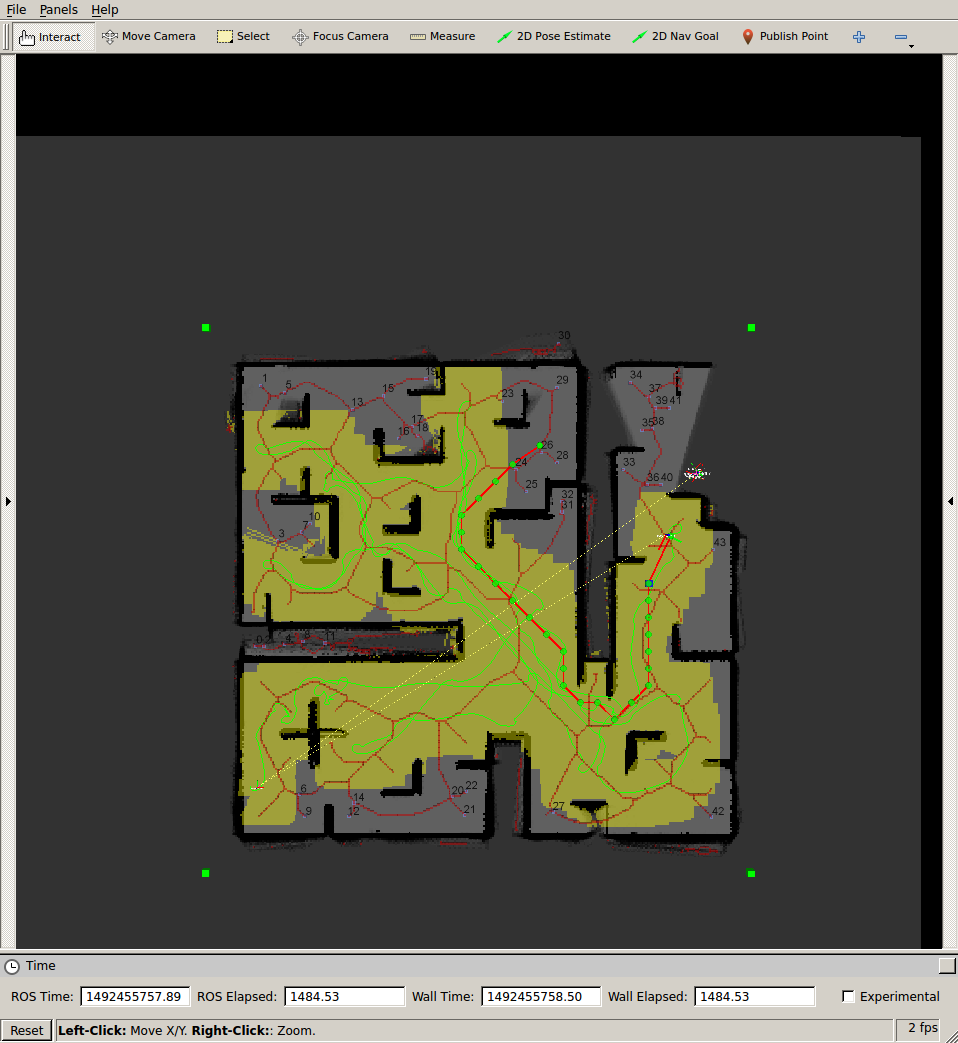
\includegraphics[width=\linewidth]{screens/random-with-path-following}
    \caption{Αποτέλεσμα των Challenge~\hyperref[section:ex3]{3} και~\hyperref[section:ex4]{4}. Path following \& obstacle avoidance με random target selector. Εικόνα από RViz~\protect\cite{rviz}.}
    \label{fig:random-with-path-following}
\end{figure}
